\section{Benchmark Design}

\subsection{Generation Pipeline}

The generator maintains a ledger whose sign convention follows normal
accounting balances: assets and expenses increase on debits, while
liabilities, equity, and revenue increase on credits.
Every transaction is applied to this ledger, and the final balance
sheet is derived directly from the resulting account state.
Revenue and expense balances are folded into Retained Earnings when the
final balance sheet is built, which makes closing-entry competence
observable in model outputs.

Transaction templates are organized by difficulty level and accounting
feature.
Lower levels emphasize basic cash bookkeeping; higher levels activate
credit transactions, debt servicing, prepaids, depreciation,
cost-of-goods-sold coupling, derived-interest calculations, and
mixed-funding purchases.
Adjustments are generated separately and applied before the statement is
prepared.
The full benchmark is deterministic given a random seed, and the
released corpus contains 2{,}500 problems.

\begin{table*}[t]
\centering
\small
\resizebox{\textwidth}{!}{%
\begin{tabular}{lrrrrl}
\toprule
Level & Problems & Avg.\ tx/problem & Avg.\ accounts & Avg.\ adjustments & Characteristic factors \\
\midrule
L1 & 500 & 7.56 & 5.18 & 0.00 & cash-only core with prepaids and basic depreciable assets \\
L2 & 750 & 14.79 & 8.38 & 0.72 & credit transactions, debt, and expiring prepaids \\
L3 & 750 & 27.39 & 11.61 & 1.68 & COGS-linked sales, accruals, depreciation, derived interest \\
L4 & 400 & 47.55 & 14.16 & 3.16 & mixed-funding purchases and dense adjustment chains \\
L5 & 100 & 79.35 & 15.22 & 4.57 & all complexity factors active in the same problem \\
\bottomrule
\end{tabular}
}
\caption{Dataset composition. Difficulty scales both the number of journal events and the number of simultaneously active accounting mechanisms.}
\label{tab:dataset-summary}
\end{table*}


Table~\ref{tab:dataset-summary} shows that difficulty corresponds to
substantive changes in bookkeeping complexity.
Average transactions increase from $7.56$ at Level~1 to $79.35$ at
Level~5, while average account support rises from $5.18$ to $15.22$.
The generator therefore scales both event count and latent bookkeeping
structure.

\begin{figure*}[t]
  \centering
  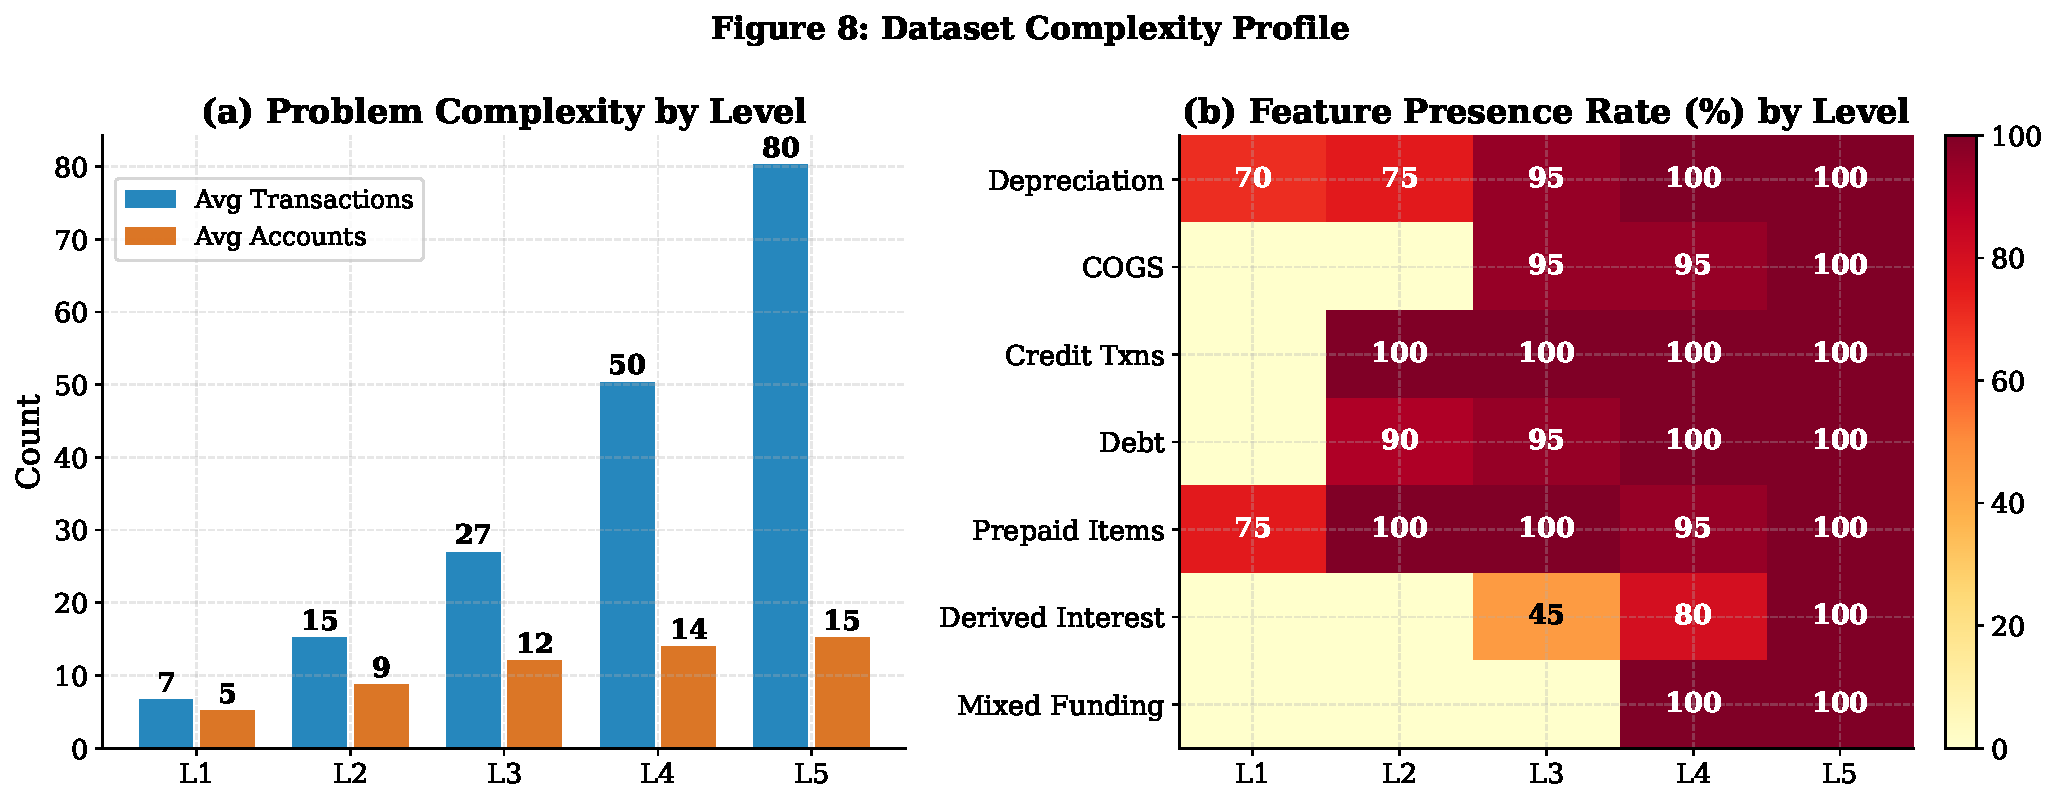
\includegraphics[width=0.95\textwidth]{../figures/F8_dataset_complexity.pdf}
  \caption{Dataset complexity profile. Panel (A) reports the mean number
    of transactions and distinct non-zero balance-sheet accounts per
    problem at each difficulty level. Panel (B) reports the percentage of
    problems at each level containing each accounting mechanism. Higher
    levels therefore increase both bookkeeping volume and mechanism
  diversity.}
  \label{fig:dataset-complexity}
\end{figure*}

Figure~\ref{fig:dataset-complexity} shows that harder levels are not
just longer prompts but introduce interacting accounting mechanisms.
Level~1 uses 5--10 cash-only transactions; Level~2 adds credit
transactions and a single adjustment; Level~3 introduces depreciation,
COGS coupling, and bad-debt provisions; Level~4 combines mixed-funded
purchases with chained adjustments; and Level~5 uses the full mechanism
set at high density (60--100 transactions, 3--5 adjustments).
Appendix~\ref{app:difficulty-samples} gives abbreviated sample problems
for each level.

\subsection{Prompted Task}

\benchmark{} evaluates whether a model can prepare a valid balance
sheet from the provided ledger state and transaction stream.
\zs{} prompting asks for a JSON answer directly with a reminder that
assets must equal liabilities plus equity.
Reflective \CoT{} prompting asks the model to reason step by step and
then emit a final JSON object after the marker
\texttt{FINAL ANSWER:}.
These are the two evaluated prompting conditions in this paper.

Appendix~\ref{app:worked-example} provides a full worked pipeline
example for this task, including the prompted input, intermediate
ledger updates, the retained-earnings closure step, and the final
expected JSON output.
Appendix~\ref{app:difficulty-samples} additionally provides abbreviated
sample problems for each of the five difficulty levels.

\subsection{Metrics and Error Taxonomy}

No single score captures this task well because a model can predict the
right account names while still violating the bookkeeping.
We therefore report the following primary metrics:
\begin{enumerate}[leftmargin=*,topsep=2pt,itemsep=2pt]
  \item \textbf{Balance accuracy (\ba{})}: a hard binary check that
    equals \(1\) only when the predicted statement satisfies
    \(|A-(L+E)| \leq 1\) currency unit.
  \item \textbf{Account-level accuracy (\ala{})}: the fraction of
    expected non-zero accounts whose predicted values fall within a
    hybrid tolerance of \(\max(\$10, 1\%\ \text{of expected value})\);
    omitted accounts count as incorrect.
  \item \textbf{Account coverage rate (\acr{})}: a structural metric that
    asks only whether the expected accounts appear anywhere in the
    output, regardless of value.
  \item \textbf{Closing-entry compliance rate (\cecr{})}: whether
    Retained Earnings is present in equity and numerically correct under
    the same hybrid tolerance; if Retained Earnings is not expected, the
    instance is treated as trivially compliant.
  \item \textbf{FinBalance Score}: a \(0\)--\(100\) weighted aggregate of
    \ba{}, \ala{}, constraint satisfaction, and normalized numerical
    error \(1-\min(\text{MAE}/50{,}000, 1)\).
\end{enumerate}

For the no-intermediate-state setting used in this paper, the composite
score assigns weights of \(0.375\) to \ba{}, \(0.3125\) to \ala{},
\(0.1875\) to constraint satisfaction, and \(0.125\) to normalized
numerical error.

Secondary diagnostics include balance error magnitude
\(|A-(L+E)|\), section placement accuracy, hallucination rate,
constraint satisfaction rate, and mean absolute / root mean squared
error over expected accounts.

The error taxonomy distinguishes arithmetic errors (wrong values),
omission errors (missing accounts), hallucinations (extra accounts),
classification errors (wrong section), and constraint violations
(\(A \neq L + E\)).
In the analysis sections we use three aggregate terms:
a \emph{factor-sensitivity analysis} measures score differences between
problems with and without a given accounting mechanism;
an \emph{account difficulty index} ranks accounts by omission and error
rates; and
a \emph{difficulty curve} traces level-wise scores, with the
coefficient of variation (CV) as a robustness summary.
